\section{Introduction}
\begin{itemize}
    \item \textbf{Integrals Involving a Parameter}
          \begin{example}
              Let $\int_0^1 Cx^3 \dd{x}$ where $C$ is a constant. Then it gives
              \begin{equation}
                  \int_0^1 Cx^3 \dd{x} = \frac{1}{4}C
              \end{equation}
              The result contains $C$.
          \end{example}
    \item Suppose we have something like
          \begin{equation}
              \int_a^b f(x,y) \dd{x} = g(y)
          \end{equation}
          and therefore $y$ is a parameter
          \begin{definition}
              A variable which is kept constant during an integration is called a parameter.
          \end{definition}
    \item         Partial integration wrt $x$

          \begin{example}
              An example of partial integration wrt $x$ is
              \begin{equation}
                  \int_0^1 x^3 y\dd{x} = y\int_0^1 x^3 \dd{x}  = \frac{1}{4}y
              \end{equation}
          \end{example}
    \item Notice the similarity between partial differentiation wrt $x$, $f_x(x,y)$ and the partial integration wrt $x$, $\int_a^b f(x,y) \dd{x}$.
    \item \textbf{Iterated Integrals} (Integral of an Integral)
    \item Consider $x=f(x,y)$ where $x\in [a,b]$, $y\in [c,d]$. This defines a rectangular region.
    \item Assume that $f(x,y)\ge 0$. This can be represented as a surface, as shown below:
          %   \begin{center}
          %       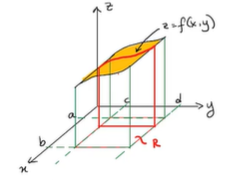
\includegraphics[width=0.6\linewidth]{L01_a.png}
          %   \end{center}
          \begin{center}
              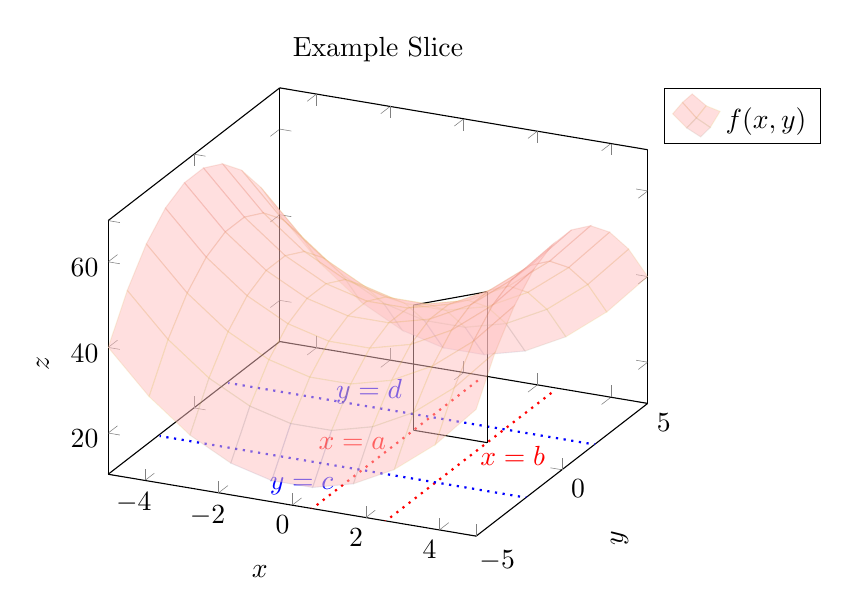
\begin{tikzpicture}
                  \begin{axis}[
                          legend pos=outer north east,
                          title=Example Slice,
                          axis lines = box,
                          colormap/hot,
                          xlabel = $x$,
                          ylabel = $y$,
                          zlabel = $z$,
                          variable = t,
                          trig format plots = rad,
                      ]
                      \draw[thick, dotted, red] (0.5,-5,10) -- (0.5,5,10) node[midway,left] {$x=a$};
                      \draw[thick, dotted, red] (2.5,-5,10) -- (2.5,5,10) node[midway,right] {$x=b$};
                      \draw[thick, dotted, blue] (5,-2,10) -- (-5,-2,10) node[midway,below left] {$y=c$};
                      \draw[thick, dotted, blue] (5,2,10) -- (-5,2,10) node[midway,above left] {$y=d$};

                      \draw[] (0.5, 1, 10) -- (2.5, 1, 10);
                      \draw[] (0.5, 1, 10) -- (0.5, 1, 39.25);
                      \draw[] (2.5, 1, 10) -- (2.5, 1, 45.25);
                      \draw[] (0.5, 1, 39.25) -- (2.5, 1, 45.25);

                      \addplot3[
                          surf,
                          samples=10,
                          color=pink,
                          opacity=0.1,
                          fill opacity=0.5
                      ]
                      {x^2-y^2+40};
                      \addlegendentry{$f(x,y)$}

                  \end{axis}
              \end{tikzpicture}
          \end{center}
          If we take the integral $\int_{y=c}^d f(x,y) \dd{y} = A(x)$, we see that the area of the slice depends on $x$.

          If we suppose that the surface has a tiny thickness $\Delta x$, then the volume is
          \begin{equation}
              \Delta V(x) = A(x) \cdot \Delta x = \left(\int_{y=c}^d f(x,y) \dd{y}\right) \Delta x
          \end{equation}
          If we break up the interval $[a,b]$ into $N$ segments
          \begin{equation}
              x_0 = a \le x_1 \le x_2 \le \dots x_{i-1} \le x_i \le \dots \le x_{N-1} \le x_N = b
          \end{equation}
          with $\Delta x_i = x_i - x_{i-1}$. We can then approximate the volume as
          \begin{equation}
              V \approx \sum_{i=1}^N \Delta V_i = \sum_{i=1}^N A(x_i)\Delta x_i
          \end{equation}
          which is known as a \textbf{Riemann sum}.
          \begin{idea}
              As we take the limit as $N\to\infty$ which implies $\Delta x_i \rightarrow 0$, we get the double integral:
              \begin{equation}
                  V = \int_a^b \int_c^d f(x,y)\dd{y}\dd{x}
              \end{equation}
              which can be determined by calculating two integrals.
          \end{idea}
    \item Similarly, we can find the volume by taking slices parallel to the $xz$ plane.

          The area of each slice is a function of $y$:
          \begin{equation}
              A(y) = \int_a^b f(x,y)\dd{x}
          \end{equation}
          so we have $\Delta V(y) = A(y) \cdot \Delta y$. Again, summing up all slices and taking the limit, we get
          \begin{equation}
              V = \int_c^d A(y) \dd{y} = \int_c^d f(x,y) \dd{x}\dd{y}
          \end{equation}
          \begin{theorem}
              \textbf{Fubini's Theorem} tells us that
              \begin{equation}
                  \int_a^b \int_c^d f(x,y) \dd{y}\dd{x} = \int_c^d \int_a^b f(x,y)\dd{x}\dd{y}
              \end{equation}
          \end{theorem}
          The analog for equality of mixed partial derivatives is known as \textbf{Clairut's Theorem.}
          \begin{example}
              Find the volume under the surface $z=x^2y$ where $x\in [1,3]$ and $y\in [0,1]$. We first form the integral by integrating wrt $y$.  We have
              \begin{align}
                  V & = \int_1^3 \int_0^1 x^2y \dd{y}\dd{x} \\
                    & = \int_1^3 x^2(1^2/2 - 0^2/2)\dd{x}   \\
                    & = \int_1^3 \frac{x^2}{2}\dd{x}        \\
                    & = \frac{13}{3}
              \end{align}
              We can also form the integral by integrate it wrt $x$:
              \begin{align}
                  V & = \int_0^1 \int_1^3 x^2y\dd{x}\dd{y} \\
                    & = \int_0^1 \frac{26}{3}y \dd{y}      \\
                    & = \frac{13}{3}
              \end{align}
              so we can confirm they give the same answer.
          \end{example}
          \begin{example}
              Evaluate the double integral of $f(x,y) = x-3y^2$ over region $R$ where
              \begin{equation}
                  R = \{(x,y)|0\le x\le 2, 1\le y\le 2\}
              \end{equation}
              To do this, we have
              \begin{align}
                  \int_0^2 \int_1^2 (x-3y^2)\dd{y}\dd{x} & = \int_0^2 (xy-y^3)\big\rvert_{y=1}^{y=2}\dd{x} \\
                                                         & = \int_0^2 (x-7)\dd{x}                          \\
                                                         & = -12
              \end{align}
          \end{example}
    \item Note that in the special case where the function $f(x,y)$ is $f(x,y)=g(x) \cdot h(y)$, then
          \begin{equation}
              \int_c^d \int_a^b f(x,y)\dd{x}\dd{y} = \int_c^d\left[h(y)\int_a^b g(x) \dd{x}\right] \dd{y} = \int_a^b g(x) \dd{x} \cdot \int_c^d h(y) \dd{y}
          \end{equation}
          This gives us a shortcut of evaluating double integrals in this form.
    \item Double integrals over general regions (What if region is non-rectangular?)

    \item \textbf{Type 1 Region} is in the form of
          \begin{equation}
              R = \{(x,y) | a\le x \le b, g_1(x) \le y \le g_2(x)\}
          \end{equation}
          Here are some examples
          %   \begin{center}
          %       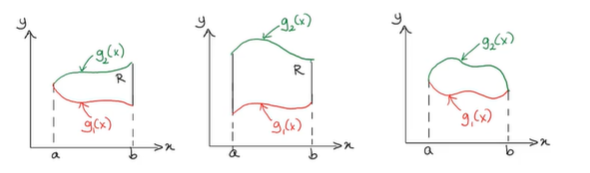
\includegraphics[width=0.6\linewidth]{L01_b.png}
          %   \end{center}
          \begin{center}
              \begin{tikzpicture}[scale=0.8]
                  \begin{axis}[
                          legend pos=outer north east,
                          title=Example of Type 1,
                          axis lines = box,
                          xmin = 0,
                          ymin = 0,
                          xmax = 3,
                          ymax = 4,
                          xlabel = $x$,
                          ylabel = $y$,
                          variable = t,
                          trig format plots = rad,
                      ]
                      \addplot [
                          domain=0.75:2.25,
                          samples=70,
                          color=blue,
                      ]
                      {0.5*(x-2)^3+3};
                      \addlegendentry{$g(x)$}
                      \addplot [
                          domain=0.75:2.25,
                          samples=70,
                          color=red,
                      ]
                      {-0.5*(x-2)^3+1+0.046875};
                      \addlegendentry{$f(x)$}
                      \draw[] (2.25, 1.0390625) -- (2.25, 3.0078125);
                  \end{axis}
              \end{tikzpicture}
              \qquad
              \begin{tikzpicture}[scale=0.8]
                  \begin{axis}[
                          legend pos=outer north east,
                          title=Example of Type 1,
                          axis lines = box,
                          xmin = 0,
                          ymin = 0,
                          xmax = 3,
                          ymax = 4,
                          xlabel = $x$,
                          ylabel = $y$,
                          variable = t,
                          trig format plots = rad,
                      ]
                      \addplot [
                          domain=0.75:2.25,
                          samples=70,
                          color=blue,
                      ]
                      {0.5*(x-2)^3+3};
                      \addlegendentry{$g(x)$}
                      \addplot [
                          domain=0.75:2.25,
                          samples=70,
                          color=red,
                      ]
                      {-0.5*(x-2)^3+1+0.046875-0.5};
                      \addlegendentry{$f(x)$}
                      \draw[] (2.25, 1.0390625-0.5) -- (2.25, 3.0078125);
                      \draw[] (0.75, 1.5234375) -- (0.75, 2.0234375);
                  \end{axis}
              \end{tikzpicture}
              \qquad
              \begin{tikzpicture}[scale=0.8]
                  \begin{axis}[
                          legend pos=outer north east,
                          title=Example of Type 1,
                          axis lines = box,
                          xmin = 0,
                          ymin = 0,
                          xmax = 3,
                          ymax = 4,
                          xlabel = $x$,
                          ylabel = $y$,
                          variable = t,
                          trig format plots = rad,
                      ]
                      \addplot [
                          domain=0.75:2.25,
                          samples=70,
                          color=blue,
                      ]
                      {-(x-1.5)^2+3};
                      \addlegendentry{$g(x)$}
                      \addplot [
                          domain=0.75:2.25,
                          samples=70,
                          color=red,
                      ]
                      {(x-1.5)^2+1.87500};
                      \addlegendentry{$g(x)$}
                  \end{axis}
              \end{tikzpicture}
          \end{center}
    \item Let's think about the case where $f(x,y)\ge 0$ on a type-1 region. Suppose we have the following illustration
        %   \begin{center}
        %       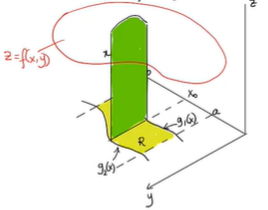
\includegraphics[width=0.6\linewidth]{L01_c.png}
        %   \end{center}
          \begin{center}
              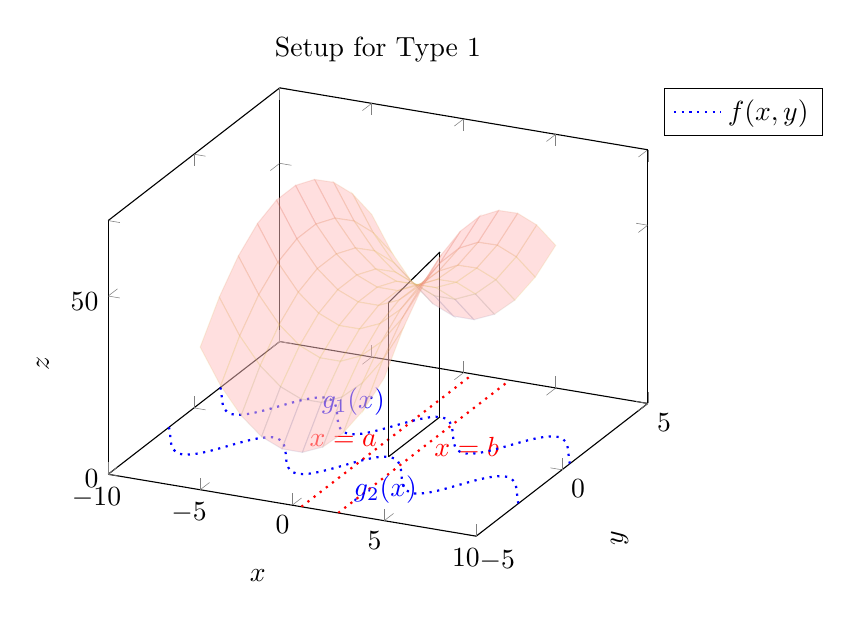
\begin{tikzpicture}
                  \begin{axis}[
                          legend pos=outer north east,
                          title=Setup for Type 1,
                          axis lines = box,
                          colormap/hot,
                          xlabel = $x$,
                          ylabel = $y$,
                          zlabel = $z$,
                          zmin=0,
                          variable = t,
                          trig format plots = rad,
                      ]
                      \draw[thick, dotted, red] (0.5,-5,0) -- (0.5,5,0) node[midway,left] {$x=a$};
                      \draw[thick, dotted, red] (2.5,-5,0) -- (2.5,5,0) node[midway,right] {$x=b$};
                      % \draw[thick, dotted, blue] (5,-2,10) -- (-5,-2,10) node[midway,below left] {$y=c$};
                      % \draw[thick, dotted, blue] (5,2,10) -- (-5,2,10) node[midway,above left] {$y=d$};
                      \addplot [
                          domain=-10:10,
                          samples=70,
                          color=blue,
                          dotted,
                          thick
                      ]
                      {sin(x)-2} node[midway, below right] {$g_2(x)$};
                      \addplot [
                          domain=-10:10,
                          samples=70,
                          color=blue,
                          dotted,
                          thick
                      ]
                      {sin(x)+1} node[midway,above left] {$g_1(x)$};
                      \draw[] (1.5, -1, 0) -- (1.5, 2, 0);
                      \draw[] (1.5, -1, 0) -- (1.5, -1, 43.25);
                      \draw[] (1.5, 2, 46.25) -- (1.5, 2, 0);
                      \draw[] (1.5, 2, 46.25) -- (1.5, -1, 43.25);

                      \addplot3[
                          surf,
                          samples=10,
                          color=pink,
                          opacity=0.1,
                          fill opacity=0.5
                      ]
                      {x^2-y^2+40};
                      \addlegendentry{$f(x,y)$}

                  \end{axis}
              \end{tikzpicture}
          \end{center}
          We find the area of slices, so
          \begin{equation}
              A(x) = \int_{g_1(x)}^{g_2(x)}f(x,y) \dd{y}
          \end{equation}
          and the volume is thus
          \begin{equation}
              V = \int_a^b A(x)\dd{X} = \int_a^b \int_{g_1(x)}^{g_2(X)} f(x,y) \dd{y}\dd{x}
          \end{equation}
    \item Type-2 regions have the form
          \begin{equation}
              R = \{(x,y) | c\le y \le d \text{ and } h_1(y) \le x \le h_2(y) \}
          \end{equation}
          In a similar way, the volume bounded by this region is
          \begin{equation}
              V = \int_c^d \int_{h_1(y)}^{h_2(y)} f(x,y) \dd{x}\dd{y}
          \end{equation}
    \item Type-3 regions are neither type-1 nor type-2. It is possible to break up the region into parts that can be classified as either type-1 or type-2:
          \begin{center}
              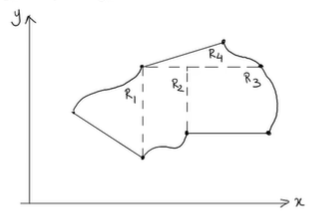
\includegraphics[width=0.6\linewidth]{L01_d.png}
          \end{center}
          \begin{idea}
              While these formulas are derived by assuming a positive volume (and thus cannot work if $f < 0$), they still work in general.
          \end{idea}
          \begin{example}
              Find the volume of the solid that lies under the surface
              \begin{equation}
                  z=f(x,y) = x^2+y^2
              \end{equation}
              and above the region $R$ in the $xy$-plane. The region $R$ is bounded by the straight line $y=2x$ and the parabola $y=x^2$.
              \begin{enumerate}
                  \item First we draw a diagram of the planar region $R$ over which the surface is defined.
                        \begin{center}
                            \begin{tikzpicture}
                                \begin{axis}[
                                        legend pos=outer north east,
                                        title=Example,
                                        axis lines = box,
                                        xlabel = $x$,
                                        ylabel = $y$,
                                        variable = t,
                                        trig format plots = rad,
                                    ]
                                    \addplot [
                                        domain=0:2,
                                        samples=70,
                                        color=blue,
                                    ]
                                    {2*x};
                                    \addlegendentry{$2x$}
                                    \addplot [
                                        domain=0:2,
                                        samples=70,
                                        color=red,
                                    ]
                                    {x^2};
                                    \addlegendentry{$x^2$}
                                \end{axis}
                            \end{tikzpicture}
                        \end{center}
                  \item We then draw a line parallel to the axis of first integration (i.e. vertical lines for integrating in the $y$-direction first)
                  \item This gives us
                        \begin{align}
                            V & = \int_{x=0}^{x=2} \int_{y=x^2}^{y=2x}f(x,y)\dd{y}\dd{x} \\
                              & = \int_0^2 \int_{x^2}^{2x} (x^2+y^2)\dd{y}\dd{x}         \\
                              & = \frac{216}{35}
                        \end{align}
              \end{enumerate}
              Alternatively, we can find the volume by integrating in the $x$ direction first. In this case, we need to obtain boundary curves in the $x=x(y)$ form:
              \begin{align}
                  y=x^2 & \implies x=\sqrt{y} \\
                  y=2x  & \implies x=y/2
              \end{align}
              This then gives us
              \begin{align}
                  V & = \int_{y=0}^{y=4} \int_{x=y/2}^{x=\sqrt{y}}f(x,y)\dd{x}\dd{y} \\
                    & = \frac{216}{35}
              \end{align}
          \end{example}
          \begin{warning}
              Do not just pick the minimum and maximum points. For example, the following is \textit{incorrect}
              \begin{equation}
                  \int_{y=0}^{y=4}\int_{x=0}^{x=2}f(x,y)\dd{x}\dd{y}
              \end{equation}
              as that corresponds with a rectangular region.
          \end{warning}
          \begin{example}
              Integrate the surface given by $z=e^{x^2}$ over the following region:
              \vspace{2mm}

              We can first integrate wrt $x$
              \begin{align}
                  V & = \in_{y=0}^{y=1}\int_{x=y}^{x=1} e^{x^2}\dd{x}\dd{y}
              \end{align}
              This is a hard problem since we don't know the anti-derivative of $e^{x^2}$. To solve this, we can first integrate wrt $y$, which gives us
              \begin{align}
                  V & = \int_{x=0}^{x=1}\int_{y=0}^{y=x}e^{x^2}\dd{y}\dd{x} & = \int_{x=0}^1 e^{x^2}y\big\rvert_{y=0}^{y=x}\dd{x} \\
                    & = \int_0^1 e^{x^2}x\dd{x}
              \end{align}
              This integral can be more easily solved using the u-sub $u=x^2$, $\dd{u}=2x\dd{x}$ to get
              \begin{equation}
                  V = \frac{1}{2}(e-1)
              \end{equation}
          \end{example}
\end{itemize}